\section{DevSecOps}

\subsection{Importancia de DevSecOps}

MisiOps guarda credenciales de acceso y el historial financiero de cada usuario: ingresos, gastos y presupuestos. Una contraseña filtrada en el repositorio, una dependencia con una vulnerabilidad crítica o una cabecera de seguridad ausente bastan para exponer esos datos y destruir la confianza en el producto. En un esquema tradicional la seguridad se revisa al final, cuando corregir es caro y el código vulnerable ya está publicado.

DevSecOps integra los controles de seguridad dentro del mismo flujo de entrega continua (\textit{shift-left}): cada cambio se analiza automáticamente en el pipeline, los hallazgos se centralizan en un único lugar con historial y ningún cambio con una alerta abierta llega a la rama de producción. En MisiOps esto se traduce en tres decisiones concretas:

\begin{itemize}
    \item \textbf{Seguridad automatizada en cada PR}: SAST, DAST, escaneo de secretos, SCA con SBOM, escaneo de imágenes y de configuración corren en GitHub Actions con versiones fijadas de cada herramienta.
    \item \textbf{Centralización}: los 11 reportes de cada corrida se importan en DefectDojo, donde se triagean, se marcan falsos positivos y se aceptan riesgos con fecha de vencimiento.
    \item \textbf{Gates}: en \texttt{main} los hallazgos bloqueantes impiden el merge; en \texttt{develop} el mismo análisis solo reporta, mediante la exención temporal EX-001 de la constitución del proyecto (vigente hasta el 2026-12-31).
\end{itemize}

La parte de seguridad se desarrolló con el mismo flujo SDD del proyecto: especificación, evaluación, plan, checklist de seguridad y tareas en \texttt{specs/011-devsecops/}, integradas mediante el PR \#130 y el PR \#132 hacia \texttt{develop}.

\subsection{Modelado de amenazas STRIDE}

El modelo de amenazas se construyó como un diagrama de flujo de datos de MisiOps con sus límites de confianza: Internet, la red Docker \texttt{public} (frontend y backend), la red Docker \texttt{private} (PostgreSQL), GitHub (repositorio y CI) y el equipo local donde corre DefectDojo con el túnel ngrok. Cada amenaza se marca sobre el componente o flujo afectado con su letra STRIDE y su identificador (Figura~\ref{fig:stride}).

\begin{figure}[H]
    \centering
    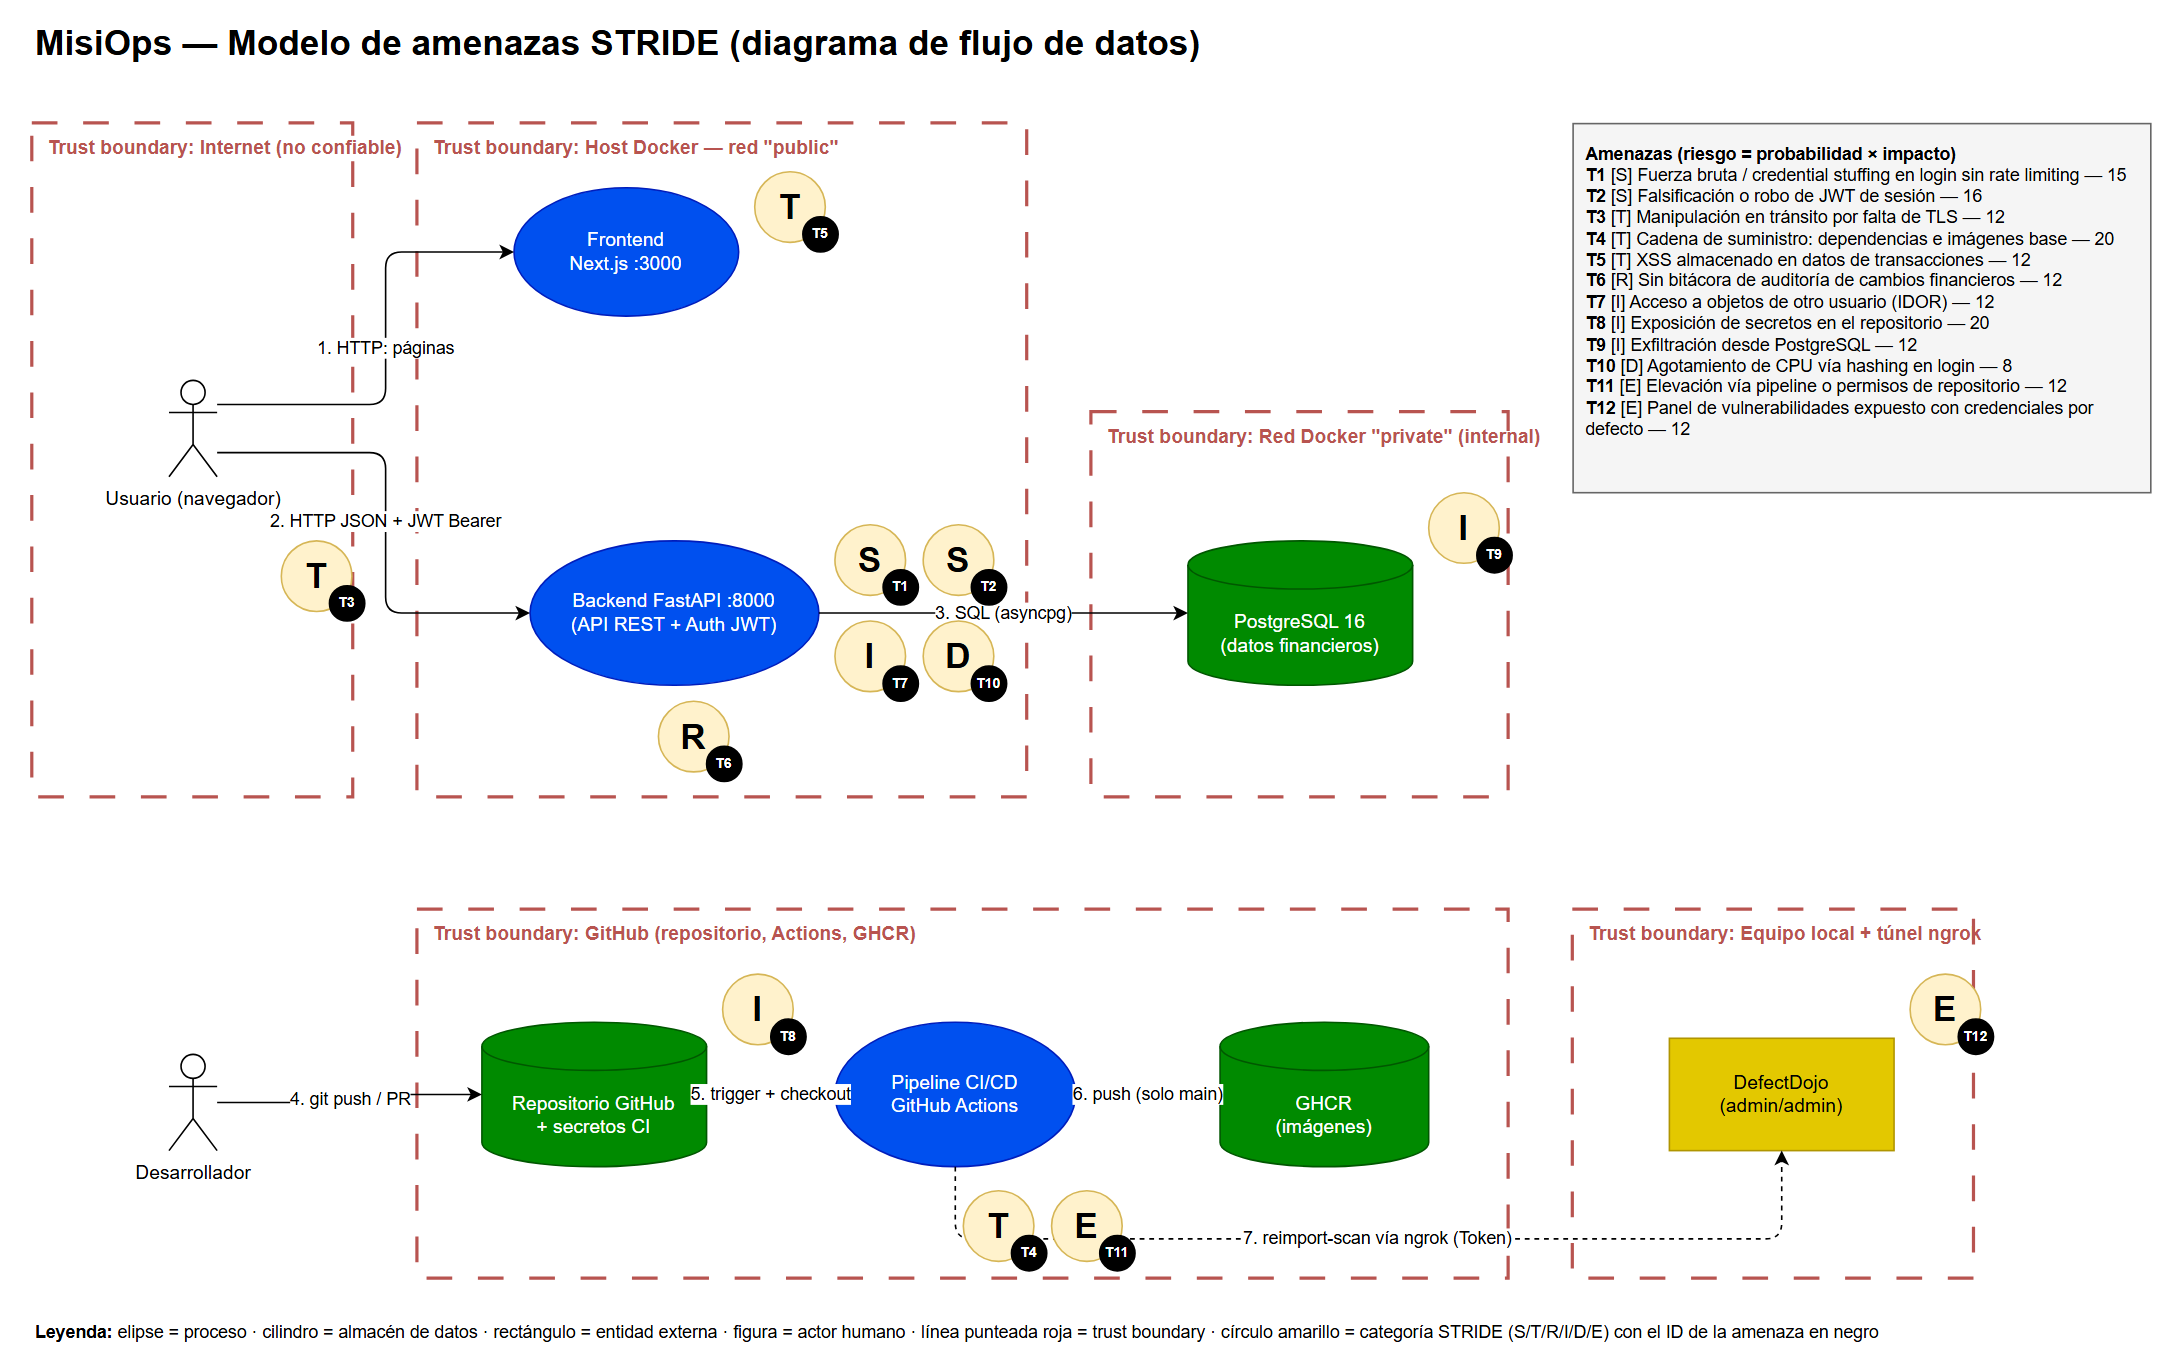
\includegraphics[width=\textwidth]{figures/devsecops/misiops-stride.png}
    \caption{Diagrama STRIDE de MisiOps con límites de confianza e identificadores de amenazas}
    \label{fig:stride}
\end{figure}

La plantilla STRIDE del curso se completó con 12 amenazas que cubren las seis categorías. Para cada una se registró probabilidad e impacto (OWASP Risk Rating, escala 1--5), riesgo inherente, controles actuales, efectividad y riesgo residual.

\begin{itemize}
    \item Diagrama editable (draw.io): \url{https://drive.google.com/file/d/1KUr076G14cM2zBuOgaE54n6_bmTbzVqY/view?usp=sharing}
    \item Plantilla STRIDE: \url{https://docs.google.com/spreadsheets/d/1e4LJ7QdhE3OWo3MIgwexaNvFtrVSTK0w/edit?usp=sharing}
    \item En el repositorio: \texttt{docs/devsecops/stride/} (\texttt{.drawio}, \texttt{.png}, \texttt{.xlsx} y \texttt{amenazas.json}).
\end{itemize}

\subsubsection{Cinco principales vulnerabilidades}

Las amenazas se ordenaron por riesgo $=$ probabilidad $\times$ impacto. En caso de empate se prioriza la que afecta credenciales o datos financieros. La Tabla~\ref{tab:stride-top5} resume las cinco principales.

\begin{table}[H]
    \centering
    \small
    \caption{Cinco amenazas STRIDE priorizadas}
    \label{tab:stride-top5}
    \begin{tabularx}{\textwidth}{@{}c l X c c X@{}}
        \toprule
        \textbf{\#} & \textbf{ID} & \textbf{Amenaza} & \textbf{STRIDE} & \textbf{P$\times$I} & \textbf{Mitigación} \\
        \midrule
        1 & T8 & Un secreto (\texttt{SECRET\_KEY}, contraseña de BD, token de DefectDojo) se sube al repositorio público o queda en el historial & I & 20 & Gitleaks y TruffleHog sobre todo el historial en CI, hook pre-commit, secretos solo en GitHub Secrets \\
        2 & T4 & Una dependencia vulnerable o una imagen base sin versión fija entra a la imagen publicada & T & 20 & SCA, SBOM y escaneo de imágenes con Trivy; \texttt{uv} fijado por digest; entrega solo si todo pasa \\
        3 & T2 & Falsificar o reutilizar un JWT si la \texttt{SECRET\_KEY} es débil o se filtra & S & 16 & Clave de al menos 32 bytes desde secretos; propuesto: rotación y revocación \\
        4 & T1 & Fuerza bruta o \textit{credential stuffing} en \texttt{/auth/login}, sin límite de intentos & S & 15 & argon2 y respuesta uniforme; propuesto: \textit{rate limiting} y bloqueo temporal \\
        5 & T7 & IDOR: cambiar el ID en \texttt{/transactions/\{id\}} para ver datos de otro usuario & I & 12 & Cada consulta filtra por el \texttt{user\_id} del token, con tests de 404 para recursos ajenos \\
        \bottomrule
    \end{tabularx}
\end{table}

\begin{enumerate}
    \item \textbf{T8 -- Fuga de secretos (Information Disclosure).} El repositorio es público y el historial de Git es permanente: un secreto subido una sola vez queda accesible aunque luego se borre. Con la \texttt{SECRET\_KEY} un atacante firma tokens válidos; con la contraseña de la base de datos accede a todos los datos financieros. Por eso el pipeline escanea todo el historial con dos detectores independientes y el hook local bloquea el commit antes de que llegue al remoto.
    \item \textbf{T4 -- Cadena de suministro (Tampering).} Las imágenes del backend y del frontend incluyen cientos de paquetes de terceros. Una versión vulnerable o una imagen base sin versión fija (\texttt{uv:latest}) puede cambiar entre dos builds sin que nadie lo note. El pipeline genera un SBOM, escanea dependencias e imágenes y publica exactamente las imágenes que fueron escaneadas.
    \item \textbf{T2 -- Suplantación con JWT (Spoofing).} La sesión depende de un JWT firmado con HS256. Si la clave es débil o se filtra, cualquiera puede emitir un token para otro usuario. La clave se genera con al menos 32 bytes y se inyecta como secreto; queda pendiente la rotación y revocación de tokens.
    \item \textbf{T1 -- Fuerza bruta en el login (Spoofing).} El endpoint de login no limita intentos. Las contraseñas se guardan con argon2 y la respuesta es uniforme para no revelar si el correo existe, pero falta \textit{rate limiting}, que queda como recomendación.
    \item \textbf{T7 -- IDOR (Information Disclosure).} Los recursos se identifican por ID. Si el backend no comprobara el dueño, bastaría cambiar el número en la URL para leer transacciones ajenas. Todas las consultas filtran por el usuario del token y existen tests que esperan 404 para recursos de otro usuario.
\end{enumerate}

T8 y T4 fueron las que más guiaron el diseño del pipeline: los escáneres de secretos y de dependencias e imágenes existen precisamente para cerrarlas.

\subsection{Análisis estático y dinámico (SAST y DAST)}

\subsubsection{Estrategias}

\begin{itemize}
    \item \textbf{SAST} (\textit{Static Application Security Testing}) analiza el código fuente sin ejecutarlo y busca patrones inseguros: inyección, uso de funciones peligrosas, criptografía débil o secretos en el código. Se ejecuta temprano y es barato, pero no ve cómo se comporta la aplicación desplegada.
    \item \textbf{DAST} (\textit{Dynamic Application Security Testing}) ataca la aplicación en ejecución desde afuera, como lo haría un atacante: revisa cabeceras, cookies, respuestas de error y la superficie de la API. Complementa al SAST porque detecta problemas de configuración que no están en el código.
\end{itemize}

\begin{table}[H]
    \centering
    \small
    \caption{Herramientas de SAST y DAST}
    \begin{tabularx}{\textwidth}{@{}l p{4.2cm} X@{}}
        \toprule
        \textbf{Tipo} & \textbf{Herramienta} & \textbf{Motivo de la elección} \\
        \midrule
        SAST & Semgrep 1.183.0 (\texttt{p/default}, \texttt{p/python}, \texttt{p/typescript}) & Cubre Python y TypeScript con una sola herramienta, tarda menos de 30 s y es la usada en el laboratorio del curso \\
        DAST & OWASP ZAP 2.17.0 (\textit{baseline} y \textit{API scan}) & El \textit{API scan} importa todos los endpoints desde \texttt{/openapi.json} y se autentica con un JWT real, así que también prueba las rutas protegidas \\
        \bottomrule
    \end{tabularx}
\end{table}

\subsubsection{Implementación y evidencia}

Ambos análisis son jobs del workflow \texttt{.github/workflows/devsecops.yml} (Anexo~\ref{anx:devsecops}):

\begin{itemize}
    \item \textbf{Job \texttt{sast}}: ejecuta Semgrep desde su imagen fijada y genera el reporte en JSON y texto. El archivo \texttt{.semgrepignore} excluye reportes archivados y dependencias.
    \item \textbf{Job \texttt{dast}}: levanta el \texttt{docker compose} del proyecto \textbf{con las mismas imágenes que luego se escanean y publican}. Las credenciales de la base de datos y la \texttt{SECRET\_KEY} se generan al vuelo y nunca se versionan. Después registra un usuario temporal, obtiene su token (enmascarado en el log) y corre dos escaneos ZAP: \textit{baseline} sobre el frontend y \textit{API scan} autenticado sobre el backend. Si ZAP no alcanza la aplicación, el job falla en lugar de reportar ``sin hallazgos''.
\end{itemize}

\begin{figure}[H]
    \centering
    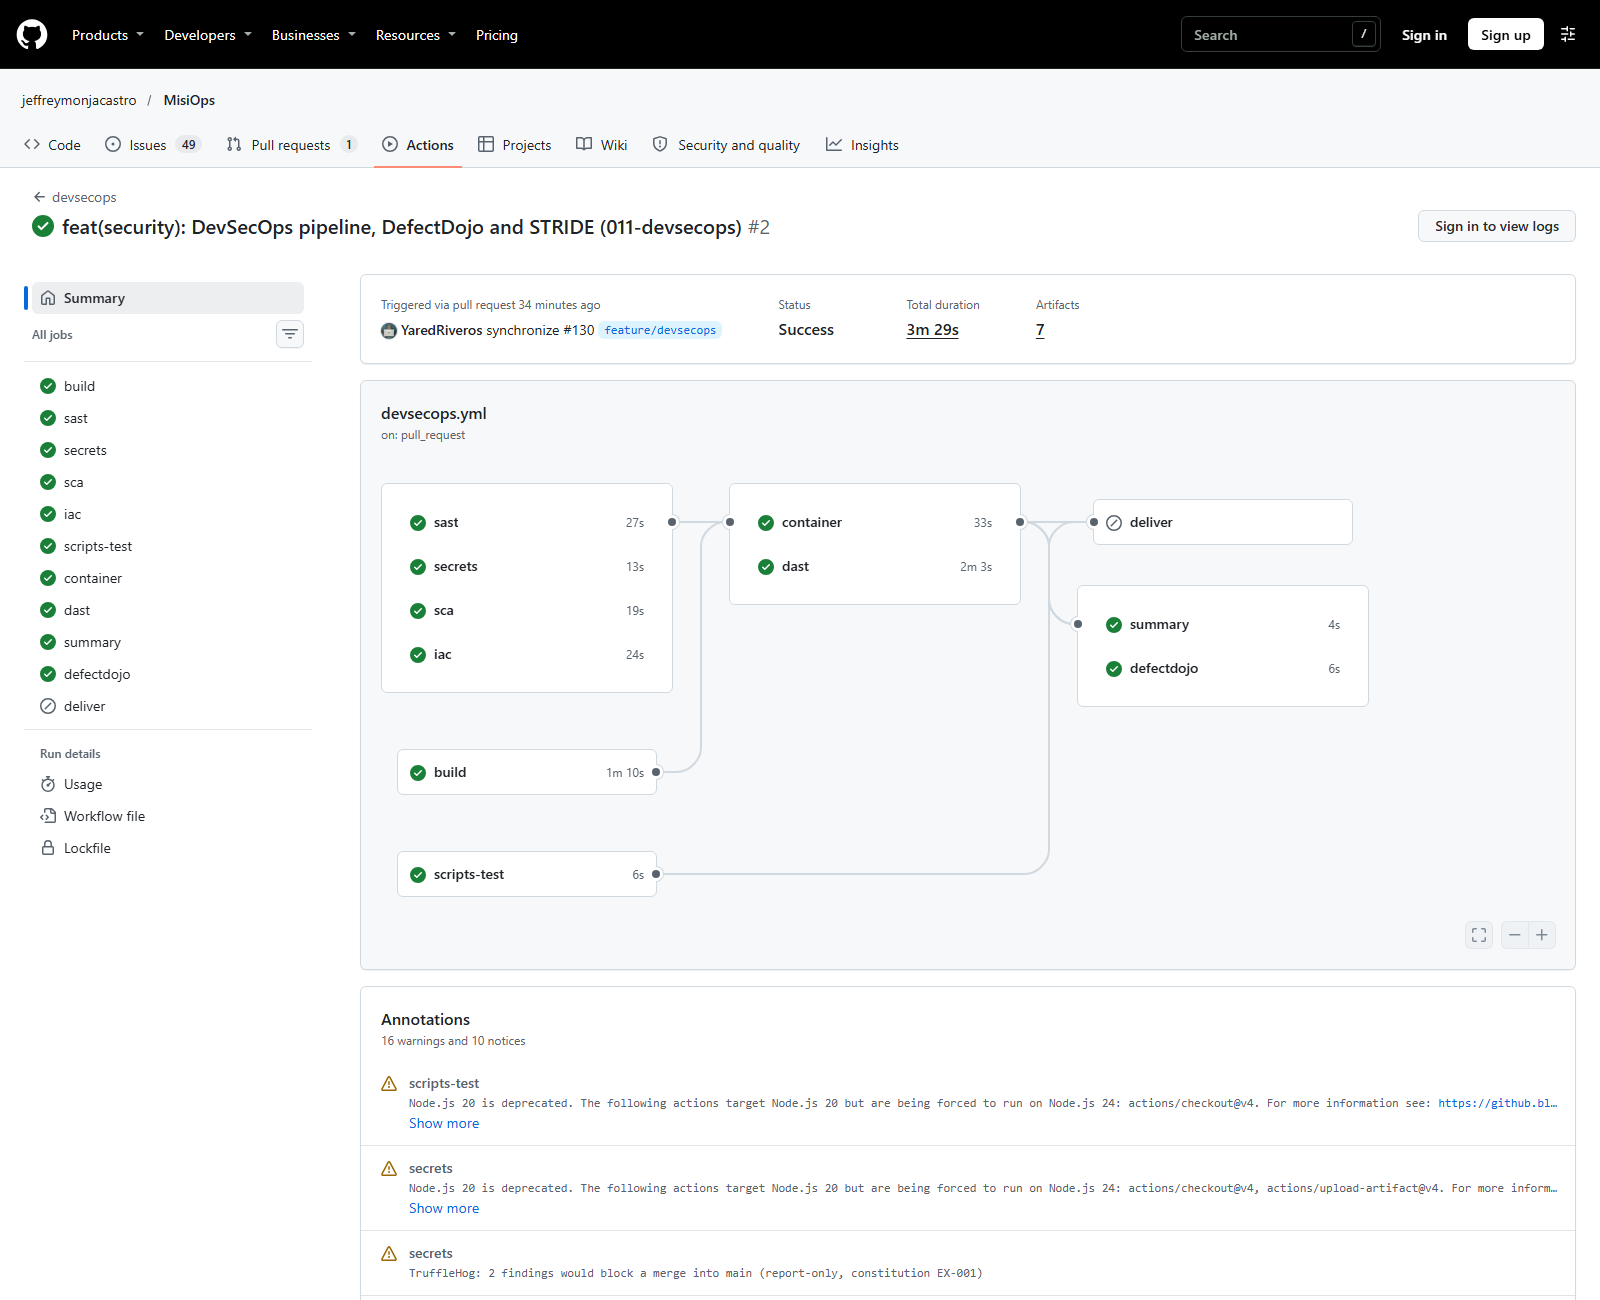
\includegraphics[width=\textwidth]{figures/devsecops/gh-actions-run.png}
    \caption{Corrida del workflow \texttt{devsecops} con los jobs de SAST, DAST y demás escaneos}
    \label{fig:gh-run}
\end{figure}

\subsubsection{Reportes generados}

En la línea base, Semgrep reportó 0 hallazgos en 76 archivos. ZAP reportó 12 alertas en el frontend (Content-Security-Policy ausente, anti-clickjacking, \texttt{X-Content-Type-Options}, \texttt{X-Powered-By}, \texttt{Permissions-Policy}, COOP/CORP) y 6 en la API. Cada corrida guarda los reportes como artefactos durante 7 días, y los de la línea base y del re-escaneo quedaron archivados en \texttt{docs/devsecops/reports/}.

\begin{figure}[H]
    \centering
    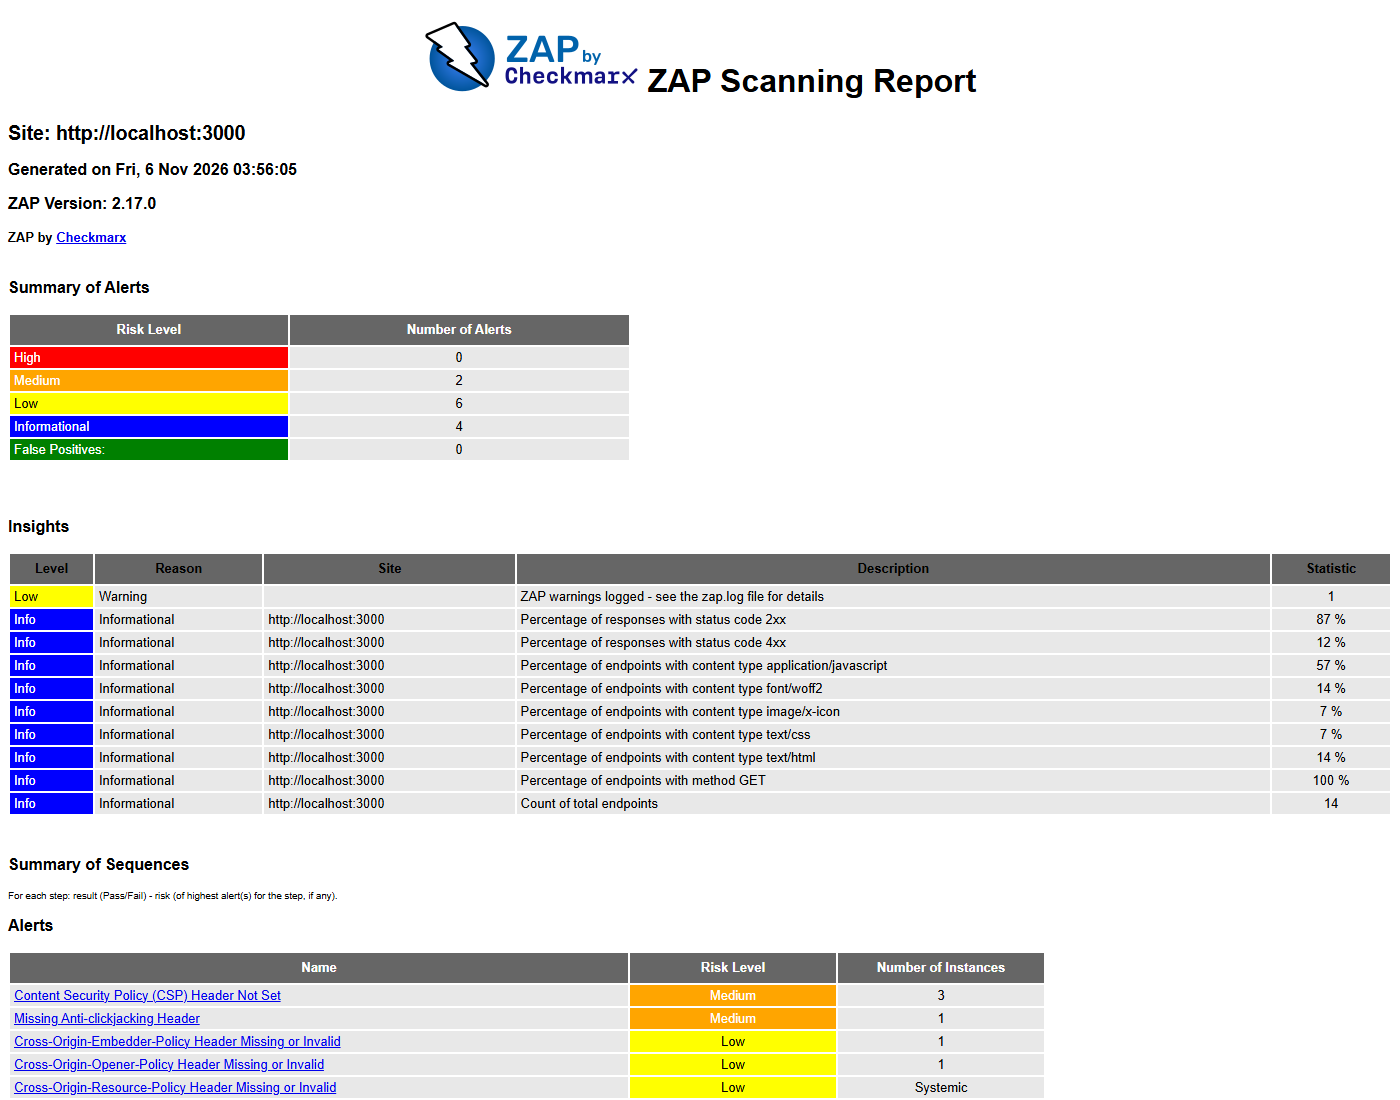
\includegraphics[width=0.9\textwidth]{figures/devsecops/zap-baseline-frontend.png}
    \caption{Reporte HTML de OWASP ZAP sobre el frontend (línea base)}
    \label{fig:zap}
\end{figure}

\subsection{Secret scanning y SCA}

\subsubsection{Estrategias}

\begin{itemize}
    \item \textbf{Secret scanning} busca credenciales (claves de API, tokens, llaves privadas, contraseñas) en el código y en todo el historial de Git, por patrones conocidos y por entropía. Lo ideal es detectarlas antes del commit, porque una vez publicadas hay que rotarlas.
    \item \textbf{SCA} (\textit{Software Composition Analysis}) inventaría las dependencias de terceros, genera un SBOM y las compara con bases de vulnerabilidades conocidas (CVE, GHSA). Se extiende a las imágenes de contenedor, que traen paquetes del sistema operativo, y a la configuración (Dockerfiles y Compose).
\end{itemize}

\begin{table}[H]
    \centering
    \small
    \caption{Herramientas de secretos, SCA, imágenes y configuración}
    \begin{tabularx}{\textwidth}{@{}p{2.4cm} p{4.2cm} X@{}}
        \toprule
        \textbf{Tipo} & \textbf{Herramienta} & \textbf{Alcance} \\
        \midrule
        Secretos (CI) & Gitleaks 8.30.1 & Patrones y entropía sobre todo el historial (\texttt{fetch-depth: 0}) \\
        Secretos (CI) & TruffleHog 3.99.8 & Segundo detector independiente sobre el historial, con verificación de credenciales vivas \\
        Secretos (local) & pre-commit (Gitleaks y \texttt{detect-private-key}) & Bloquea el commit antes de que llegue al repositorio \\
        SCA y SBOM & Trivy 0.76.1 \texttt{fs} & \texttt{backend/uv.lock} y \texttt{frontend/pnpm-lock.yaml}, más un SBOM CycloneDX \\
        Imágenes & Trivy \texttt{image} & Imágenes backend y frontend construidas en el job, más \texttt{postgres} \\
        Configuración & Trivy \texttt{config} y Semgrep \texttt{p/docker-compose} & Dockerfiles y \texttt{docker-compose.yaml} \\
        \bottomrule
    \end{tabularx}
\end{table}

\subsubsection{Implementación y evidencia}

Los jobs \texttt{secrets}, \texttt{sca}, \texttt{container} e \texttt{iac} forman parte del mismo workflow. A nivel local, \texttt{.pre-commit-config.yaml} y \texttt{.githooks/pre-commit} ejecutan Gitleaks sobre lo que está en \textit{staging}. La Figura~\ref{fig:precommit} muestra el hook bloqueando un commit con una clave AWS de prueba.

\begin{figure}[H]
    \centering
    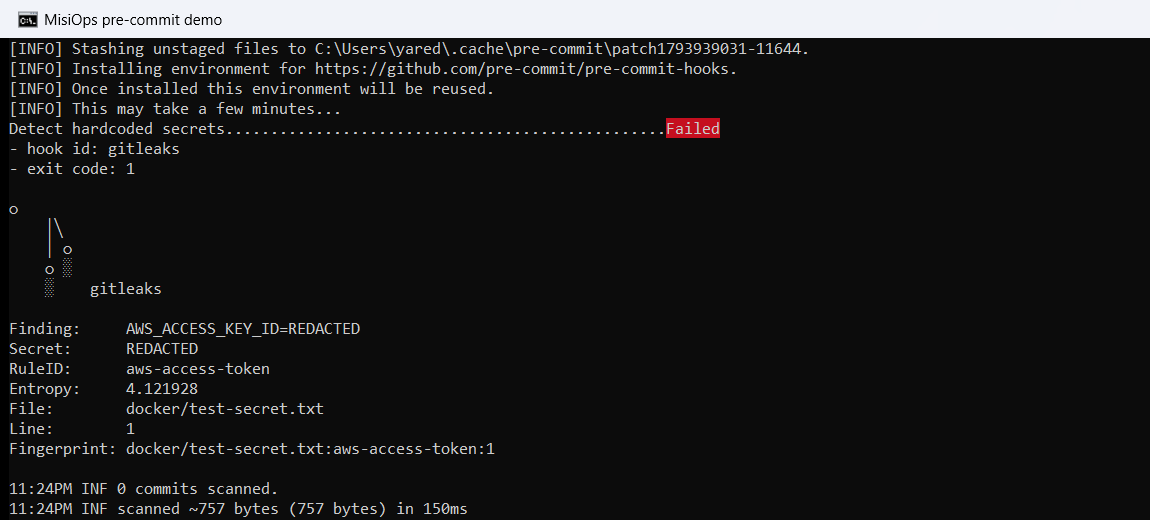
\includegraphics[width=0.9\textwidth]{figures/devsecops/precommit-bloqueo.png}
    \caption{El hook pre-commit bloquea un commit que contiene un secreto}
    \label{fig:precommit}
\end{figure}

\subsubsection{Reportes generados}

\begin{itemize}
    \item \textbf{Secretos}: en la línea base, Gitleaks reportó 4 hallazgos y TruffleHog 2. Tras revisarlos uno por uno, todos eran falsos positivos: nombres de claves de \texttt{localStorage}, la clave AWS de ejemplo del quickstart, un hash de \texttt{uv.lock} y datos de imagen de un diagrama. Quedaron en las listas de excepciones (\texttt{.gitleaks.toml}, \texttt{security/trufflehog-exclude.txt}) con justificación y fecha de revisión.
    \item \textbf{SCA}: Trivy encontró \textbf{7 CRITICAL y 9 HIGH} en las dependencias: Next.js 16.3.4, certifi, dnspython, sharp, source-map-js y un \texttt{package-lock.json} de npm obsoleto que duplicaba hallazgos.
    \item \textbf{Imágenes}: 7 hallazgos bloqueantes en la imagen backend, 64 en la frontend y 170 en \texttt{postgres:16.3}.
\end{itemize}

Los reportes están en \texttt{docs/devsecops/reports/baseline/} (\texttt{trivy-deps.txt}, \texttt{sbom.cdx.json}, \texttt{gitleaks.json}, \texttt{trufflehog.json} y los \texttt{trivy-image-*.json}).

\subsection{DefectDojo}

\subsubsection{Descripción}

DefectDojo es una plataforma open source de gestión de vulnerabilidades (OWASP). Importa los reportes de más de 200 escáneres, los normaliza en hallazgos con severidad, elimina duplicados entre corridas y permite gestionar su ciclo de vida: activo, mitigado, falso positivo o riesgo aceptado. En MisiOps se usa la versión 3.4.202, desplegada en local con Docker Compose, con esta jerarquía:

\begin{center}
    \textit{Product Type} ``Aplicaciones Web'' $\rightarrow$ \textit{Product} ``MisiOps'' $\rightarrow$ \textit{Engagement} ``CI - \textless rama\textgreater'' $\rightarrow$ un \textit{Test} por reporte
\end{center}

\subsubsection{Conexión con GitHub Actions}

\begin{itemize}
    \item DefectDojo corre en un equipo del equipo de trabajo y se expone a GitHub Actions mediante un túnel ngrok con dominio fijo.
    \item El job \texttt{defectdojo} lee los secretos de repositorio \texttt{DEFECTDOJO\_URL} y \texttt{DEFECTDOJO\_TOKEN}. Luego ejecuta \texttt{security/scripts/upload\_to\_defectdojo.sh} (Anexo~\ref{anx:upload}), que sube cada reporte con \texttt{POST /api/v2/reimport-scan/}.
    \item El archivo \texttt{security/scripts/reports.tsv} asocia cada reporte con su parser de DefectDojo y con un título de \textit{Test} propio (por ejemplo ``Trivy - image backend''). Con un título compartido, como en el script del laboratorio, la importación de un reporte cerraba los hallazgos de otro.
    \item La reimportación con \texttt{close\_old\_findings} no duplica hallazgos y marca como mitigados los que ya no aparecen.
    \item Si el túnel no está activo, la subida se omite sin romper los escaneos. Luego \texttt{security/scripts/import\_run.sh \textless run-id\textgreater} descarga los artefactos de esa corrida y los importa desde la máquina local.
    \item El script tiene 37 casos de prueba (\texttt{security/tests/test\_upload\_to\_defectdojo.sh}), que corren en CI en el job \texttt{scripts-test}.
\end{itemize}

En la corrida \href{https://github.com/jeffreymonjacastro/MisiOps/actions/runs/42334876339}{42334876339}, el log del job \texttt{defectdojo} muestra \texttt{ok:} para los 11 reportes.

\subsubsection{Capturas de la aplicación}

\begin{figure}[H]
    \centering
    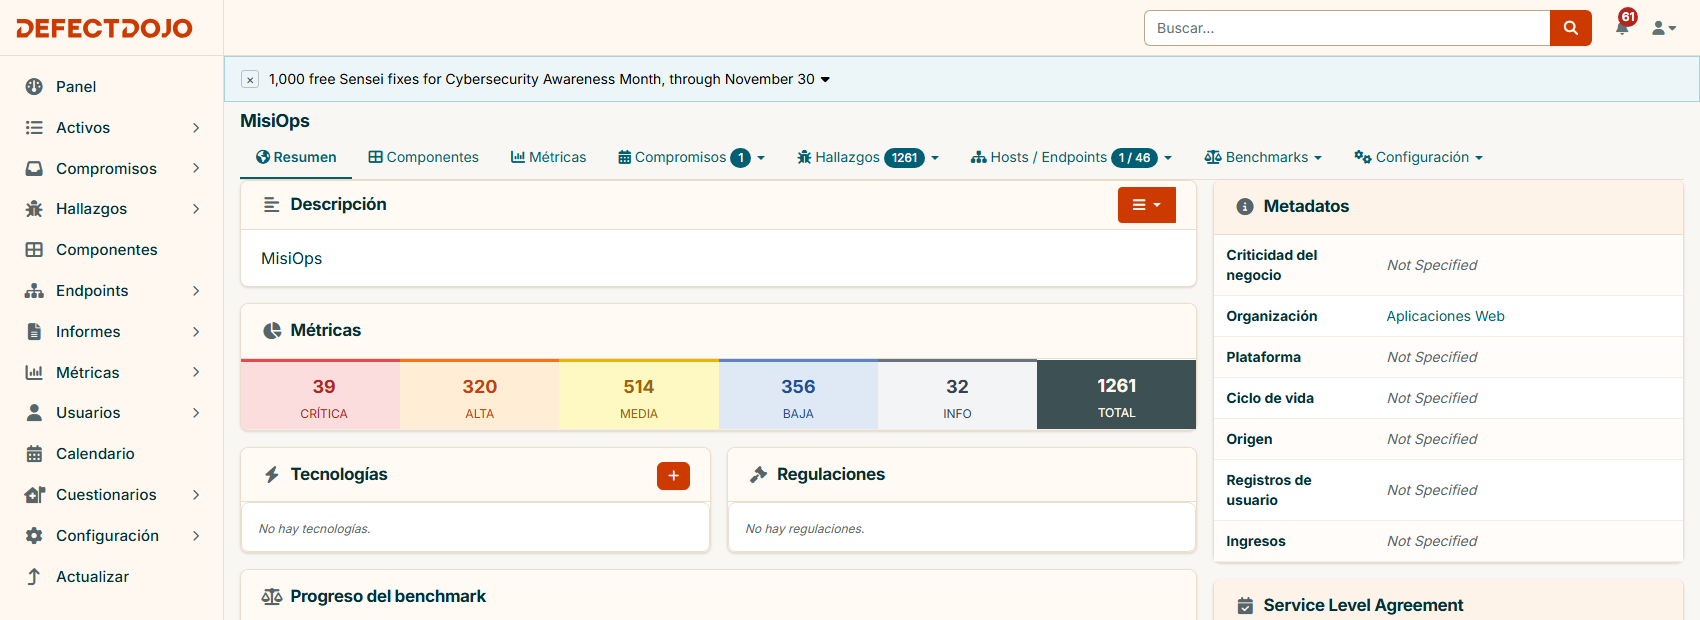
\includegraphics[width=\textwidth]{figures/devsecops/dd-baseline-producto.png}
    \caption{Producto MisiOps en DefectDojo (línea base)}
    \label{fig:dd-producto}
\end{figure}

\begin{figure}[H]
    \centering
    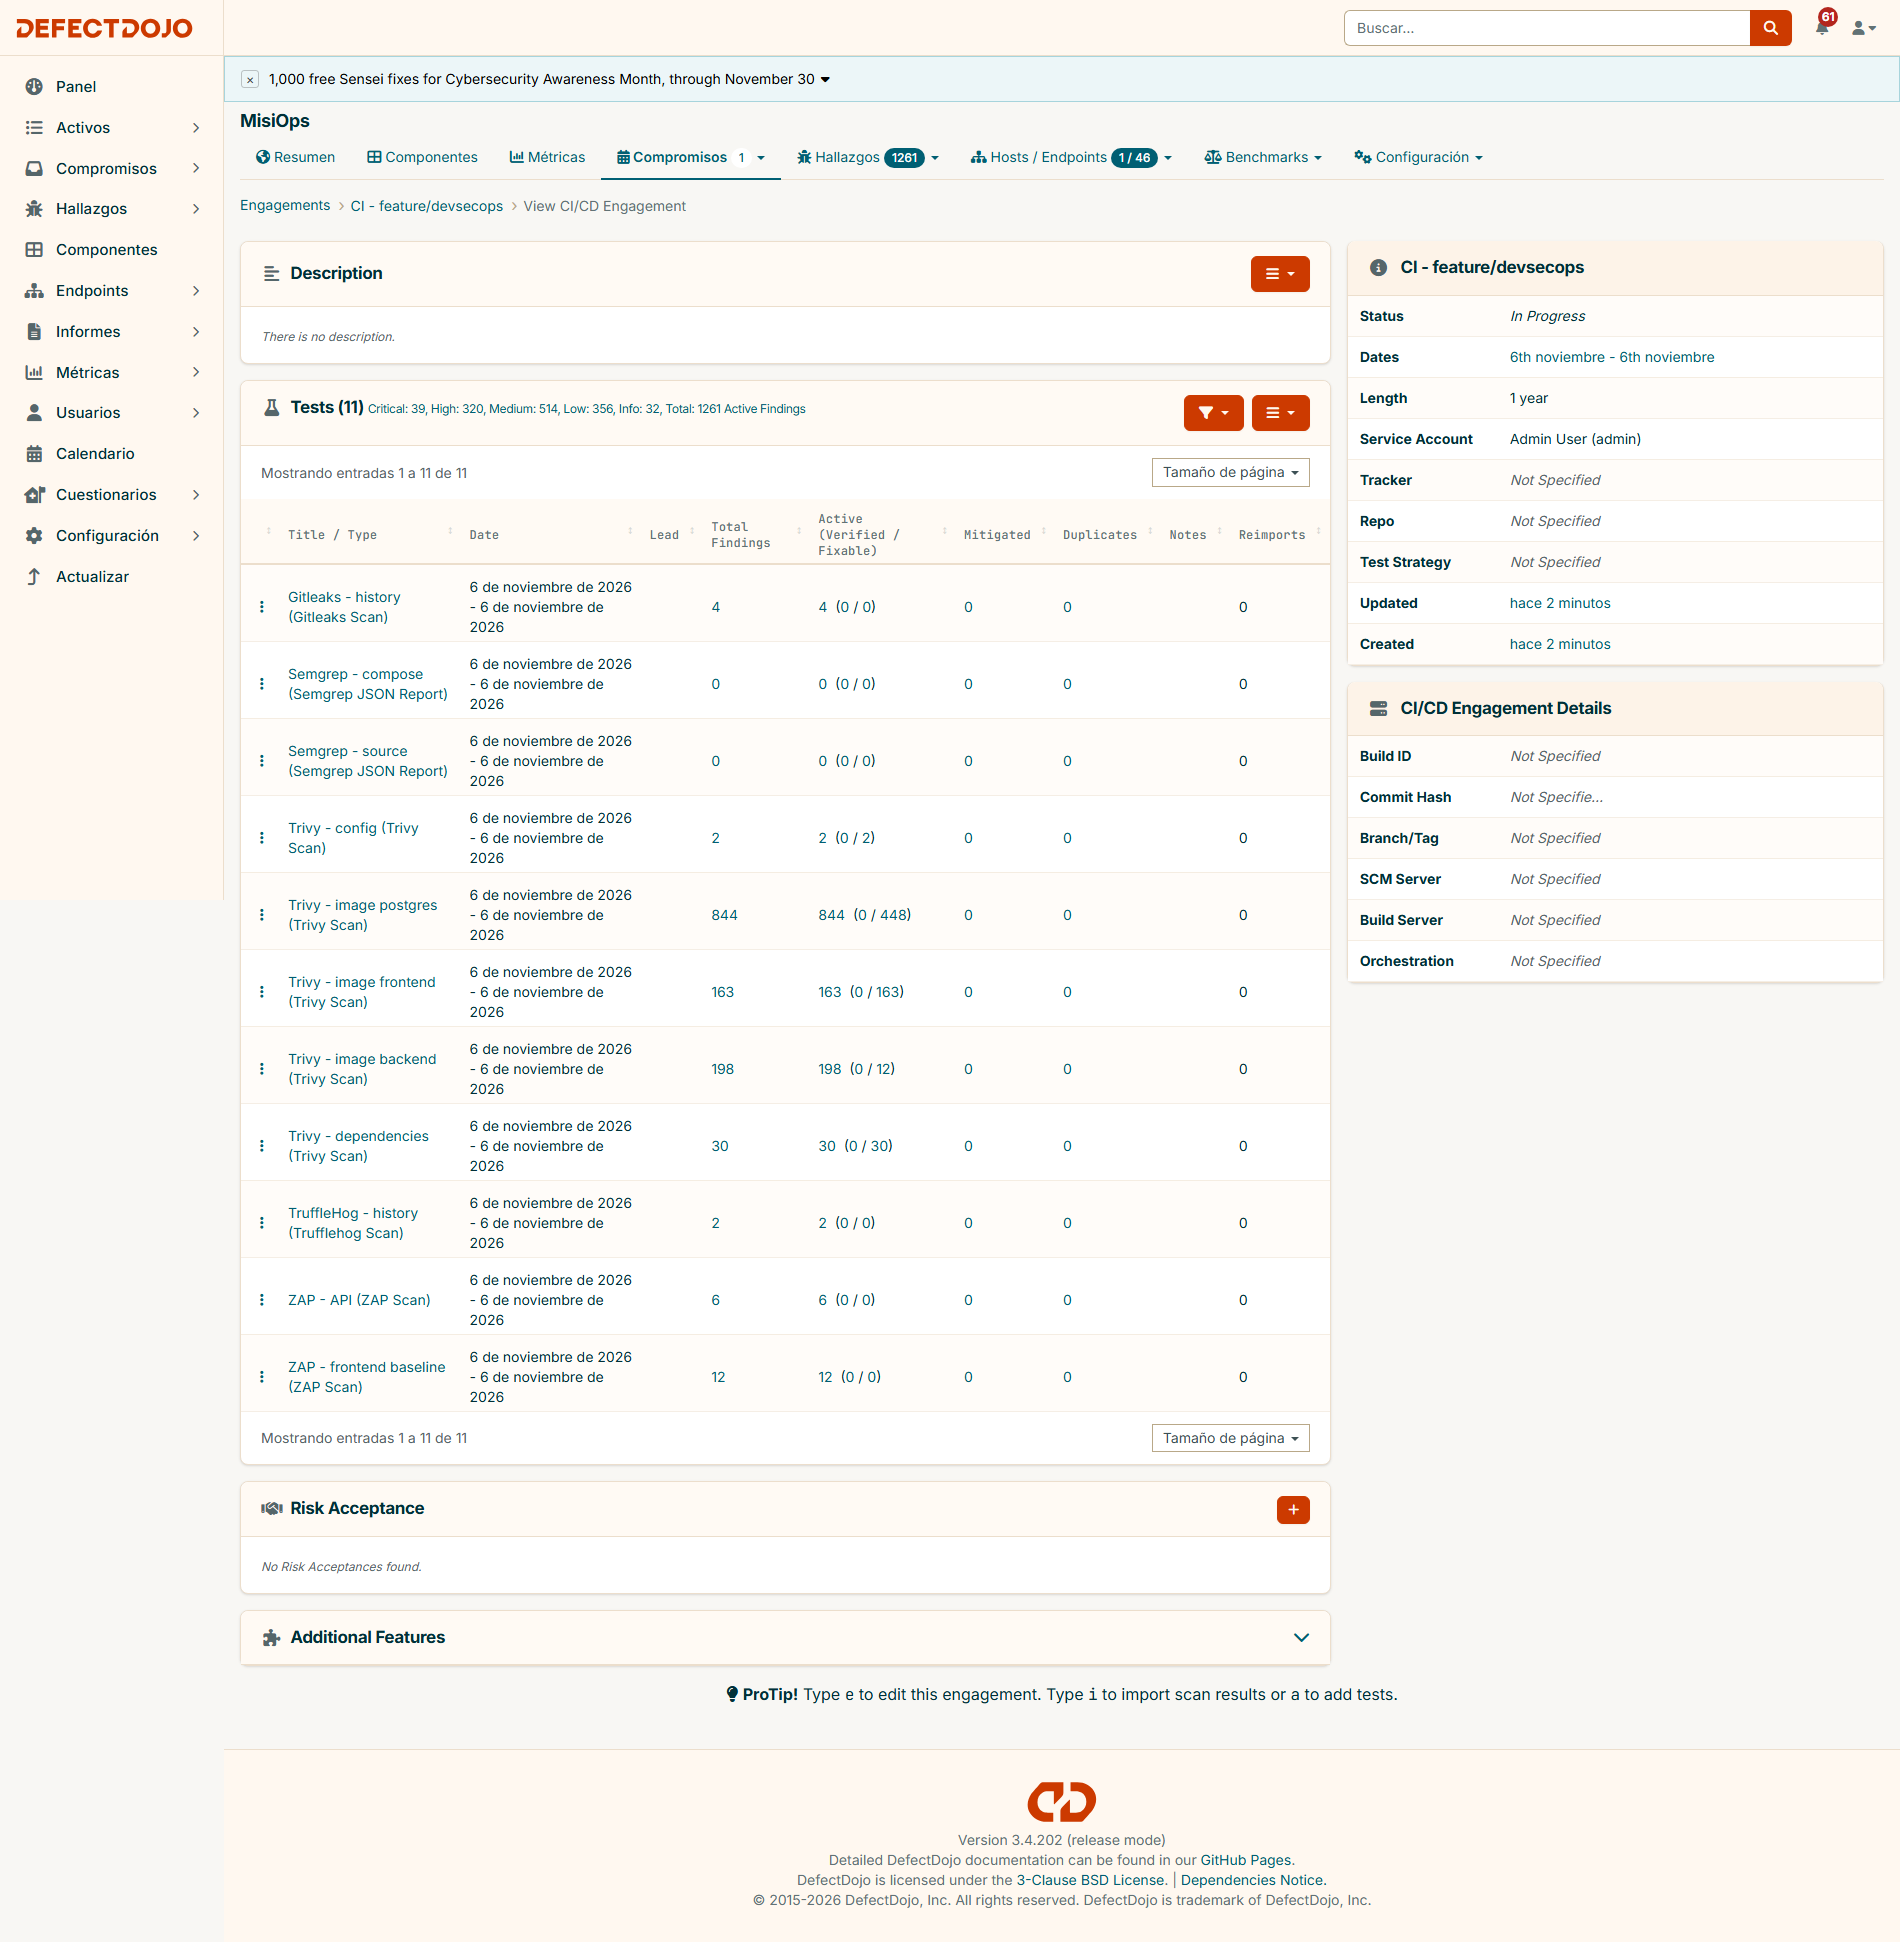
\includegraphics[width=\textwidth]{figures/devsecops/dd-baseline-engagement.png}
    \caption{Engagement de CI con los 11 tests importados (línea base)}
    \label{fig:dd-engagement}
\end{figure}

\begin{figure}[H]
    \centering
    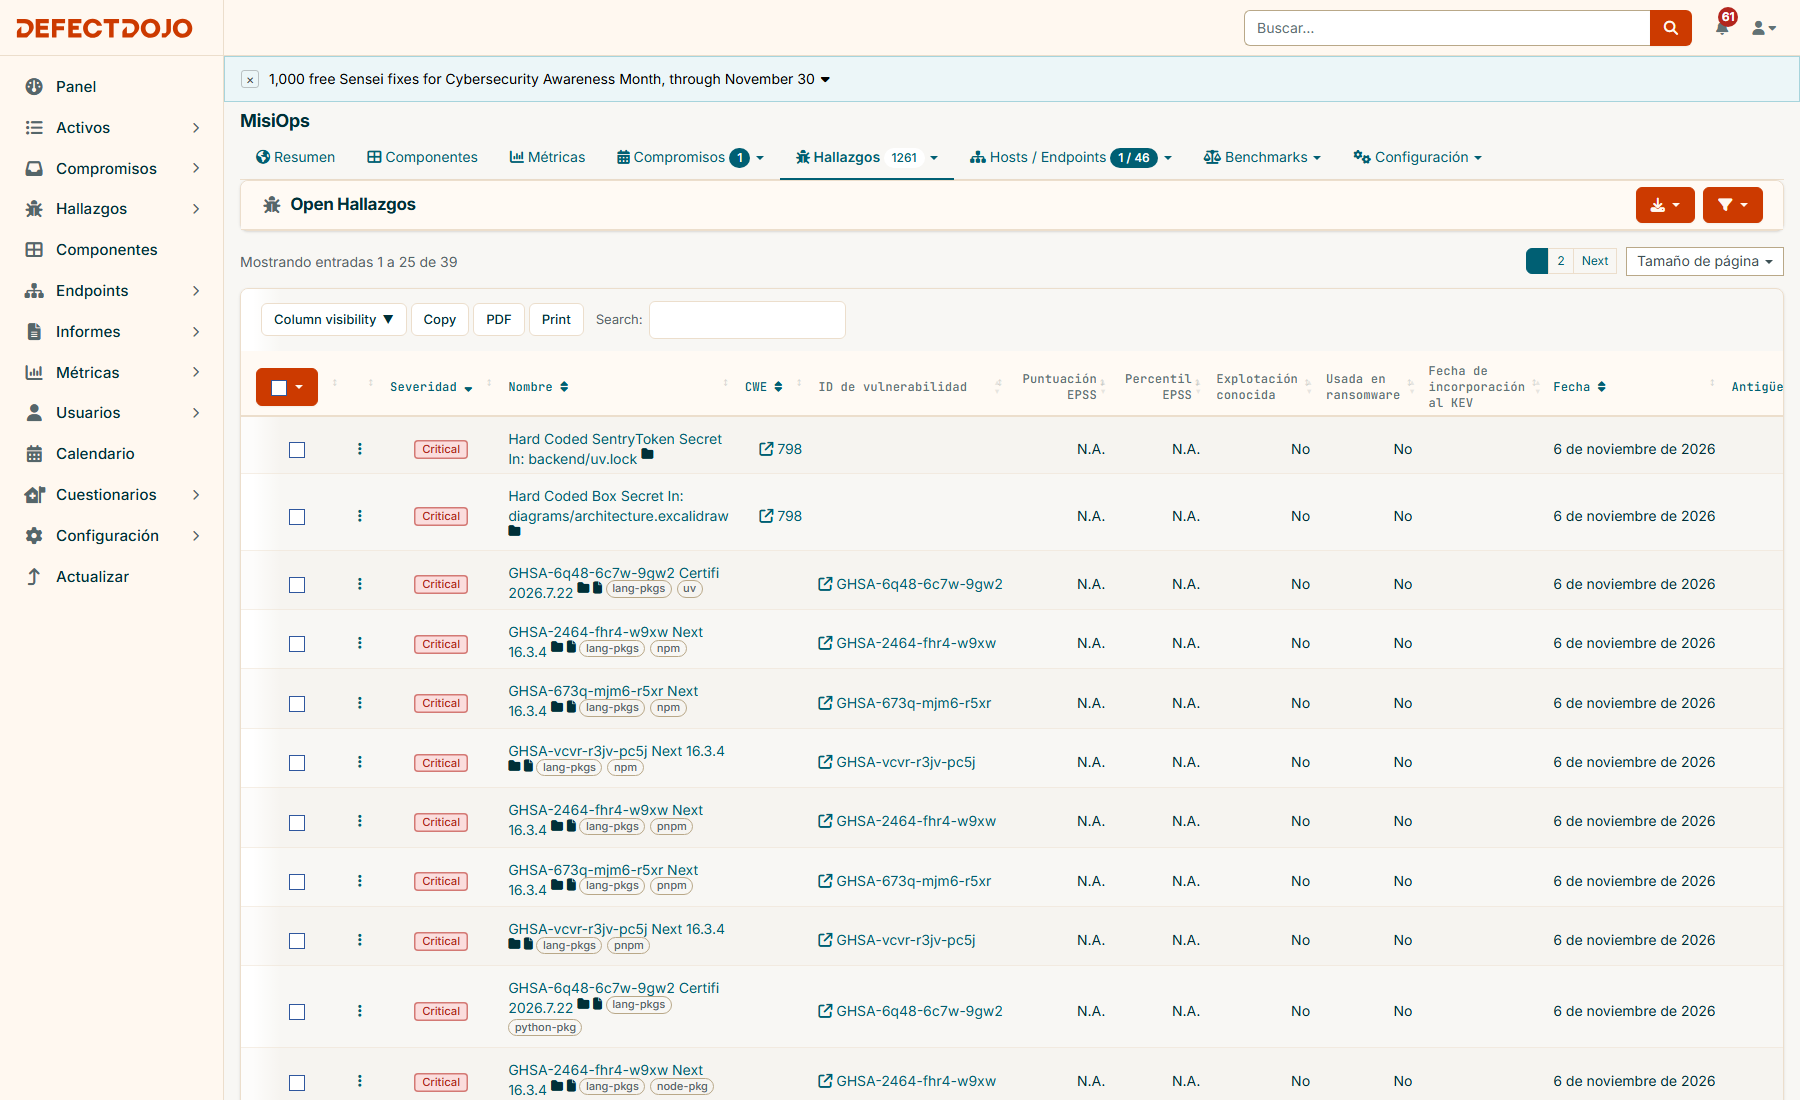
\includegraphics[width=\textwidth]{figures/devsecops/dd-baseline-criticos.png}
    \caption{Hallazgos críticos de la línea base en DefectDojo}
    \label{fig:dd-criticos}
\end{figure}

\subsection{Tabla de mitigaciones}

Los hallazgos se ordenan por severidad. Dentro de una misma severidad, primero va lo que afecta credenciales o datos financieros (amenazas T1, T2, T7, T8 y T9). Cada mitigación cita el commit del PR \#130 que la aplica.

\begin{table}[H]
    \centering
    \scriptsize
    \caption{Hallazgos priorizados y mitigaciones aplicadas}
    \label{tab:mitigaciones}
    \begin{tabularx}{\textwidth}{@{}L{1.25cm} Y L{1.25cm} L{1.65cm} Y L{1.55cm}@{}}
        \toprule
        \textbf{ID} & \textbf{Descripción} & \textbf{Severidad} & \textbf{Herramienta} & \textbf{Mitigación (commit)} & \textbf{Estado} \\
        \midrule
        CRIT-001 & Next.js 16.3.4 con GHSA-vcvr-r3jv-pc5j, GHSA-673q-mjm6-r5xr y GHSA-2464-fhr4-w9xw, en el lockfile y en la imagen frontend & Critical & Trivy SCA e imagen & Subir a \texttt{next} 16.4.5 y eliminar el \texttt{package-lock.json} obsoleto (\texttt{5883661}) & Mitigado \\
        CRIT-002 & certifi 2026.7.22 (GHSA-6q48-6c7w-9gw2), almacén de CA de las conexiones TLS del backend & Critical & Trivy SCA e imagen & Subir a certifi 2026.10.23 (\texttt{5883661}) & Mitigado \\
        CRIT-003 & \texttt{postgres:16.3} con 24 CRITICAL del SO (p.\,ej. libgnutls30 CVE-2026-33845) y 170 hallazgos corregibles & Critical & Trivy imagen & Usar \texttt{postgres:16.15-bookworm} (\texttt{15d7400}) & Mitigado (3 sin fix publicado) \\
        HIGH-001 & PyJWT 2.14.0 (PYSEC-2026-4141, PYSEC-2026-4183), librería de firma de los JWT (T2) & High & pip-audit y Trivy imagen & Subir a pyjwt 2.15.1 (\texttt{fd970da}) & Mitigado \\
        HIGH-002 & \texttt{pip} de la imagen backend trae urllib3, msgpack y setuptools vulnerables & High & Trivy imagen & Desinstalar pip y fijar \texttt{uv} por versión y digest (\texttt{15d7400}) & Mitigado \\
        HIGH-003 & npm y corepack en la imagen frontend (cross-spawn, glob, minimatch) y OpenSSL de Alpine & High & Trivy imagen & Etapa final sin npm ni corepack y con \texttt{apk upgrade} (\texttt{15d7400}) & Mitigado \\
        HIGH-004 & 4 hallazgos de Gitleaks y 2 de TruffleHog en el historial (T8) & High & Gitleaks, TruffleHog & Revisión manual y excepción documentada (\texttt{add48cc}); hook pre-commit & Falso positivo \\
        HIGH-005 & dnspython CVE-2026-114605, sharp GHSA-wq5f-xc86-pv6w, source-map-js CVE-2026-93749 & High & Trivy SCA & Actualizar dependencias directas y transitivas (\texttt{5883661}) & Mitigado \\
        HIGH-006 & 26 CVE de la stdlib de Go en \texttt{gosu} (imagen oficial de postgres) & High & Trivy imagen & \texttt{.trivyignore.yaml} con justificación y vencimiento & Riesgo aceptado \\
        MED-001 & Sin Content-Security-Policy en el frontend (ZAP 10038), habilita XSS (T5) & Medium & ZAP baseline & CSP con \texttt{default-src 'self'} y \texttt{frame-ancestors 'none'} (\texttt{43c0621}) & Mitigado \\
        MED-002 & Sin protección anti-clickjacking (ZAP 10020) & Medium & ZAP baseline & \texttt{X-Frame-Options: DENY} (\texttt{43c0621}) & Mitigado \\
        LOW-001 & Faltan \texttt{X-Content-Type-Options}, \texttt{Permissions-Policy}, COOP/CORP y sobra \texttt{X-Powered-By} & Low & ZAP baseline y API & Cabeceras en \texttt{next.config.ts} y middleware en \texttt{backend/main.py}, con tests (\texttt{43c0621}) & Mitigado \\
        \bottomrule
    \end{tabularx}
\end{table}

\subsection{Técnicas de seguridad y mitigación: antes y después}

\textbf{Antes}, el CI solo tenía lint, tests, build, una prueba de integración con Docker y \texttt{pip-audit}. No había escaneo de secretos, de imágenes ni de configuración, tampoco DAST. Los resultados no se reunían en ningún lugar y nada impedía integrar un cambio inseguro.

\textbf{Después}, cada corrida produce 11 reportes, se centralizan en DefectDojo y un gate impide llegar a \texttt{main} con alertas abiertas. Las técnicas aplicadas fueron:

\begin{itemize}
    \item \textbf{Actualización de dependencias} con fix publicado (Next.js, certifi, PyJWT, dnspython, sharp, source-map-js).
    \item \textbf{Reducción de la superficie de las imágenes}: el backend sin \texttt{pip} y con \texttt{uv} fijado por digest; el frontend sin npm ni corepack; \texttt{postgres} actualizado a una versión parcheada; y \texttt{apt-get upgrade} en la imagen del backend (PR \#180) para que los parches del SO no esperen a la imagen base.
    \item \textbf{Cabeceras de seguridad HTTP} en frontend y backend (CSP, anti-clickjacking, \texttt{nosniff}, \texttt{Permissions-Policy}, COOP/CORP), cubiertas por 7 tests nuevos.
    \item \textbf{Prevención de secretos} desde el commit local y doble detector en CI.
    \item \textbf{Gestión explícita de excepciones}: cada falso positivo o riesgo aceptado vive en el archivo de excepciones de su herramienta, con justificación y fecha de revisión, y se refleja en DefectDojo como \textit{False Positive} o \textit{Risk Acceptance}.
\end{itemize}

La línea base es la corrida \href{https://github.com/jeffreymonjacastro/MisiOps/actions/runs/42159225729}{42159225729} (commit \texttt{ff7ba32}) y el re-escaneo es la corrida \href{https://github.com/jeffreymonjacastro/MisiOps/actions/runs/42162904886}{42162904886} (commit \texttt{a628e9d}), ambas con las mismas versiones y reglas.

\begin{table}[H]
    \centering
    \small
    \caption{Hallazgos activos en DefectDojo antes y después de remediar}
    \label{tab:antes-despues}
    \begin{tabular}{@{}lrrrr@{}}
        \toprule
        \textbf{Severidad} & \textbf{Antes} & \textbf{Después} & \textbf{Cerrados (\textit{Mitigated})} & \textbf{Reducción} \\
        \midrule
        Critical & 39 & 3 & 39 & $-$92\,\% \\
        High & 320 & 93 & 274 & $-$71\,\% \\
        Medium & 514 & 284 & 441 & $-$45\,\% \\
        Low & 356 & 241 & 290 & $-$32\,\% \\
        Info & 32 & 20 & 19 & $-$38\,\% \\
        \midrule
        \textbf{Total} & \textbf{1261} & \textbf{641} & \textbf{1063} & \textbf{$-$49\,\%} \\
        \bottomrule
    \end{tabular}
\end{table}

La columna ``Después'' incluye hallazgos nuevos de las imágenes actualizadas que aún no tienen fix publicado; por eso ``antes menos cerrados'' no coincide exactamente con ``después''. Lo que decide el merge son los hallazgos \textbf{bloqueantes} de cada gate, que bajaron de 263 a 0:

\begin{table}[H]
    \centering
    \small
    \caption{Hallazgos que bloquean el merge a \texttt{main}}
    \begin{tabular}{@{}lrr@{}}
        \toprule
        \textbf{Reporte} & \textbf{Antes} & \textbf{Después} \\
        \midrule
        Trivy dependencias & 16 & 0 \\
        Trivy imagen backend & 7 & 0 \\
        Trivy imagen frontend & 64 & 0 \\
        Trivy imagen postgres & 170 & 0 \\
        Gitleaks y TruffleHog & 6 & 0 \\
        Semgrep, Trivy config y ZAP (High) & 0 & 0 \\
        \midrule
        \textbf{Total} & \textbf{263} & \textbf{0} \\
        \bottomrule
    \end{tabular}
\end{table}

\begin{figure}[H]
    \centering
    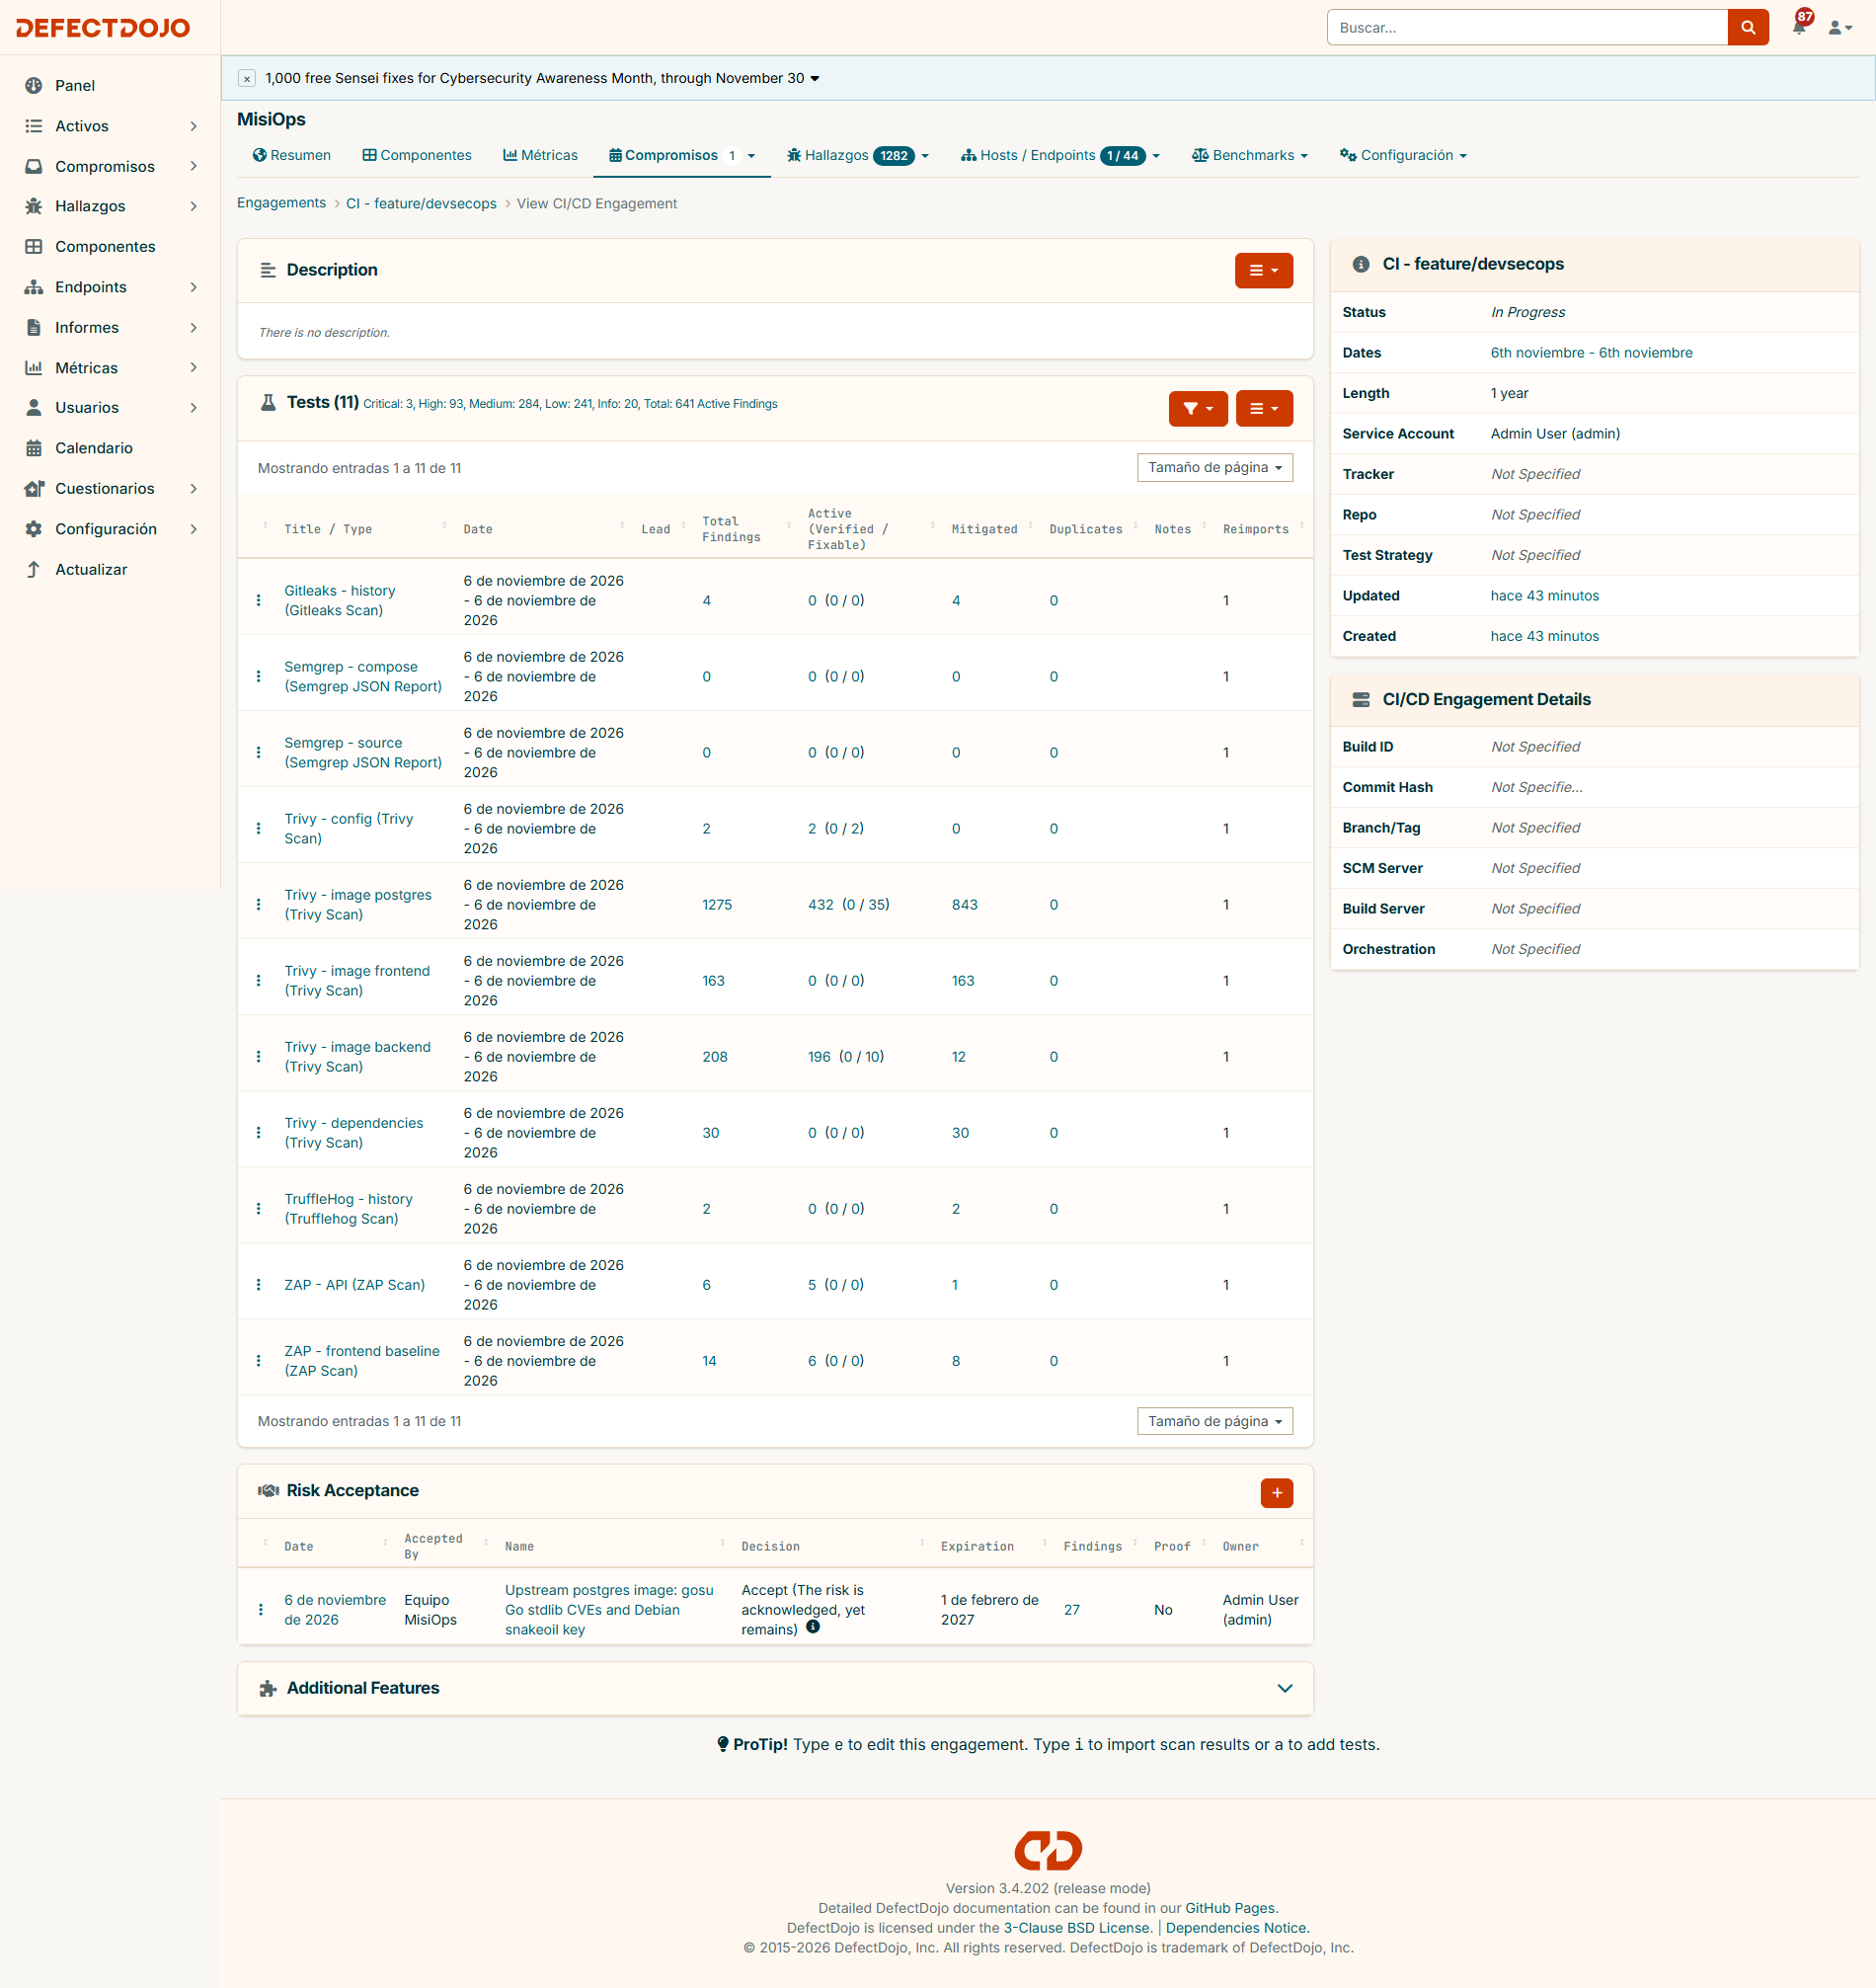
\includegraphics[width=\textwidth]{figures/devsecops/dd-rescan-engagement.png}
    \caption{Engagement después de remediar, con el panel de riesgos aceptados}
    \label{fig:dd-rescan}
\end{figure}

\begin{figure}[H]
    \centering
    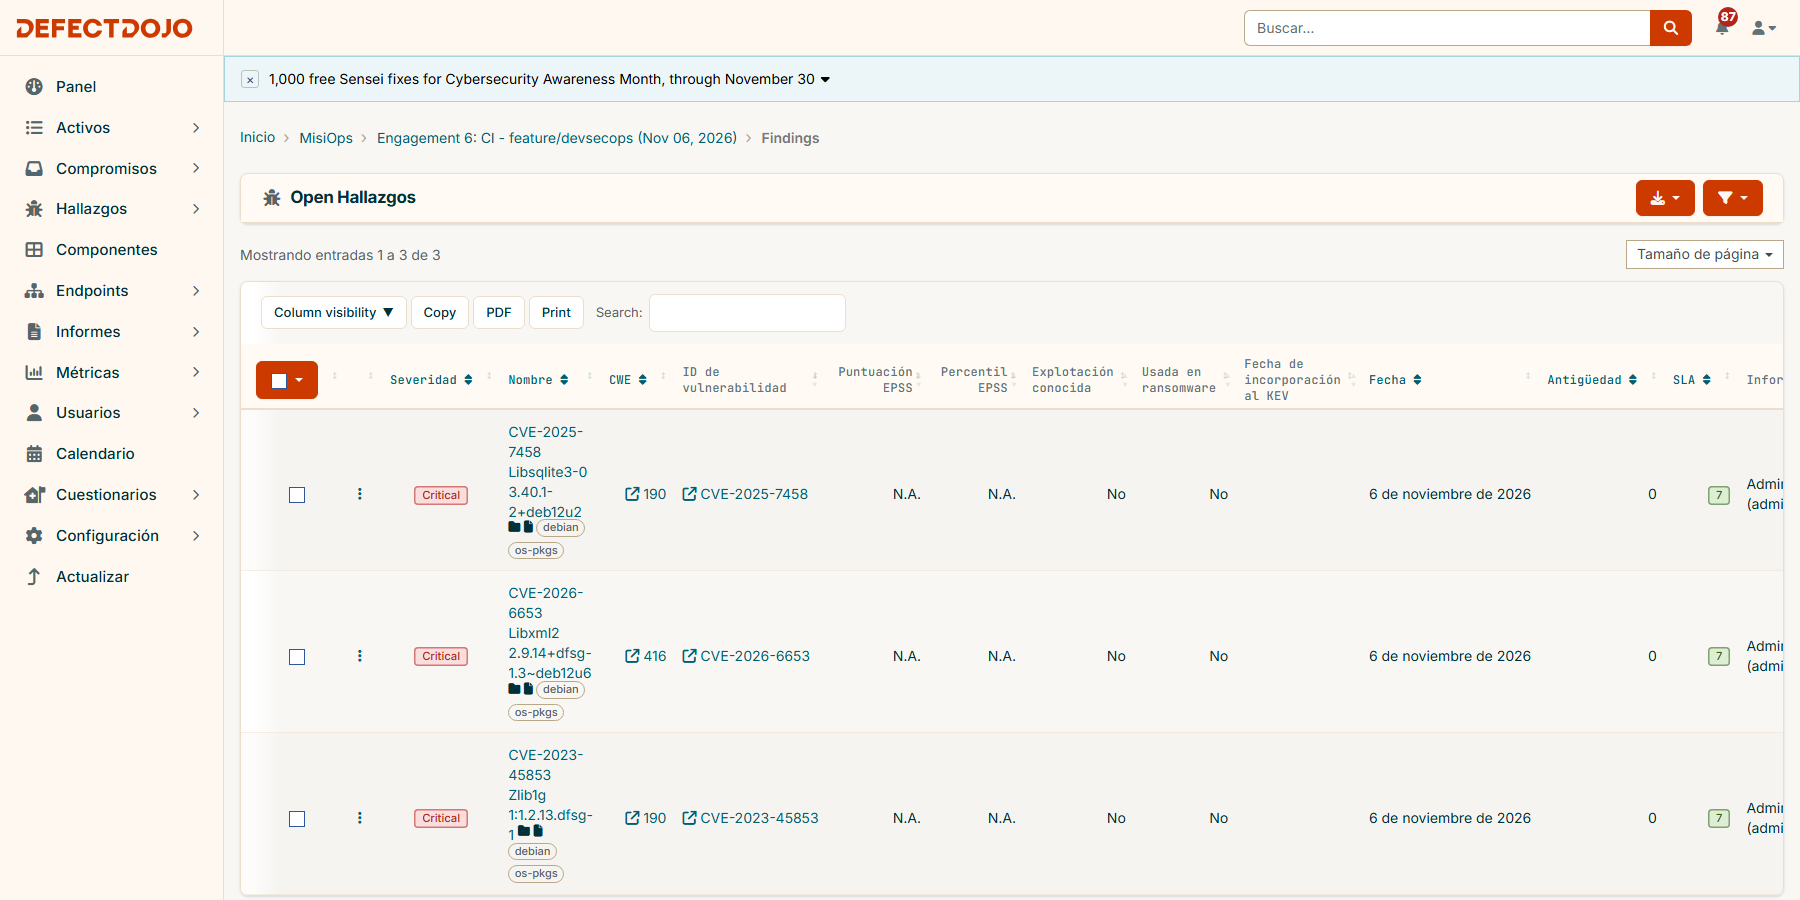
\includegraphics[width=\textwidth]{figures/devsecops/dd-rescan-criticos.png}
    \caption{Críticos abiertos tras el re-escaneo: solo quedan 3 del SO de postgres sin fix publicado}
    \label{fig:dd-rescan-crit}
\end{figure}

Las suites existentes siguen en verde (123 tests del backend y 42 del frontend), igual que lint, build e integración.

\subsection{Pipeline DevSecOps en GitHub Actions}

El workflow \texttt{devsecops.yml} corre en cada PR y en cada push a \texttt{develop} y \texttt{main} (Figura~\ref{fig:pipeline}):

\begin{enumerate}
    \item \textbf{Local}: hook pre-commit (Gitleaks y \texttt{detect-private-key}) y hook pre-push (artefactos SDD).
    \item \textbf{build}: construye una sola vez las imágenes backend y frontend y las guarda como artefacto.
    \item \textbf{En paralelo}: \texttt{sast}, \texttt{secrets}, \texttt{sca}, \texttt{iac} y \texttt{scripts-test}. Cuando termina \texttt{build}, también \texttt{container} (Trivy sobre las 3 imágenes) y \texttt{dast} (ZAP sobre el stack levantado con esas imágenes).
    \item \textbf{Gate por herramienta} (\texttt{security/scripts/gate.sh}): bloquea en \texttt{main} y solo reporta en \texttt{develop}.
    \item \textbf{summary} (tabla en el resumen de la corrida) y \textbf{defectdojo} (reimportación).
    \item \textbf{deliver}: solo en push a \texttt{main} y solo si todos los gates pasaron. Publica en GHCR \textbf{las mismas} imágenes escaneadas.
\end{enumerate}

En paralelo siguen corriendo los workflows de calidad que ya existían: \texttt{backend-ci} (ruff, pytest, pip-audit), \texttt{frontend-ci} (eslint, tests, build), \texttt{docker-integration} y el \texttt{SDD Pipeline Enforcer}. La corrida completa tarda unos 4 minutos.

\begin{figure}[H]
    \centering
    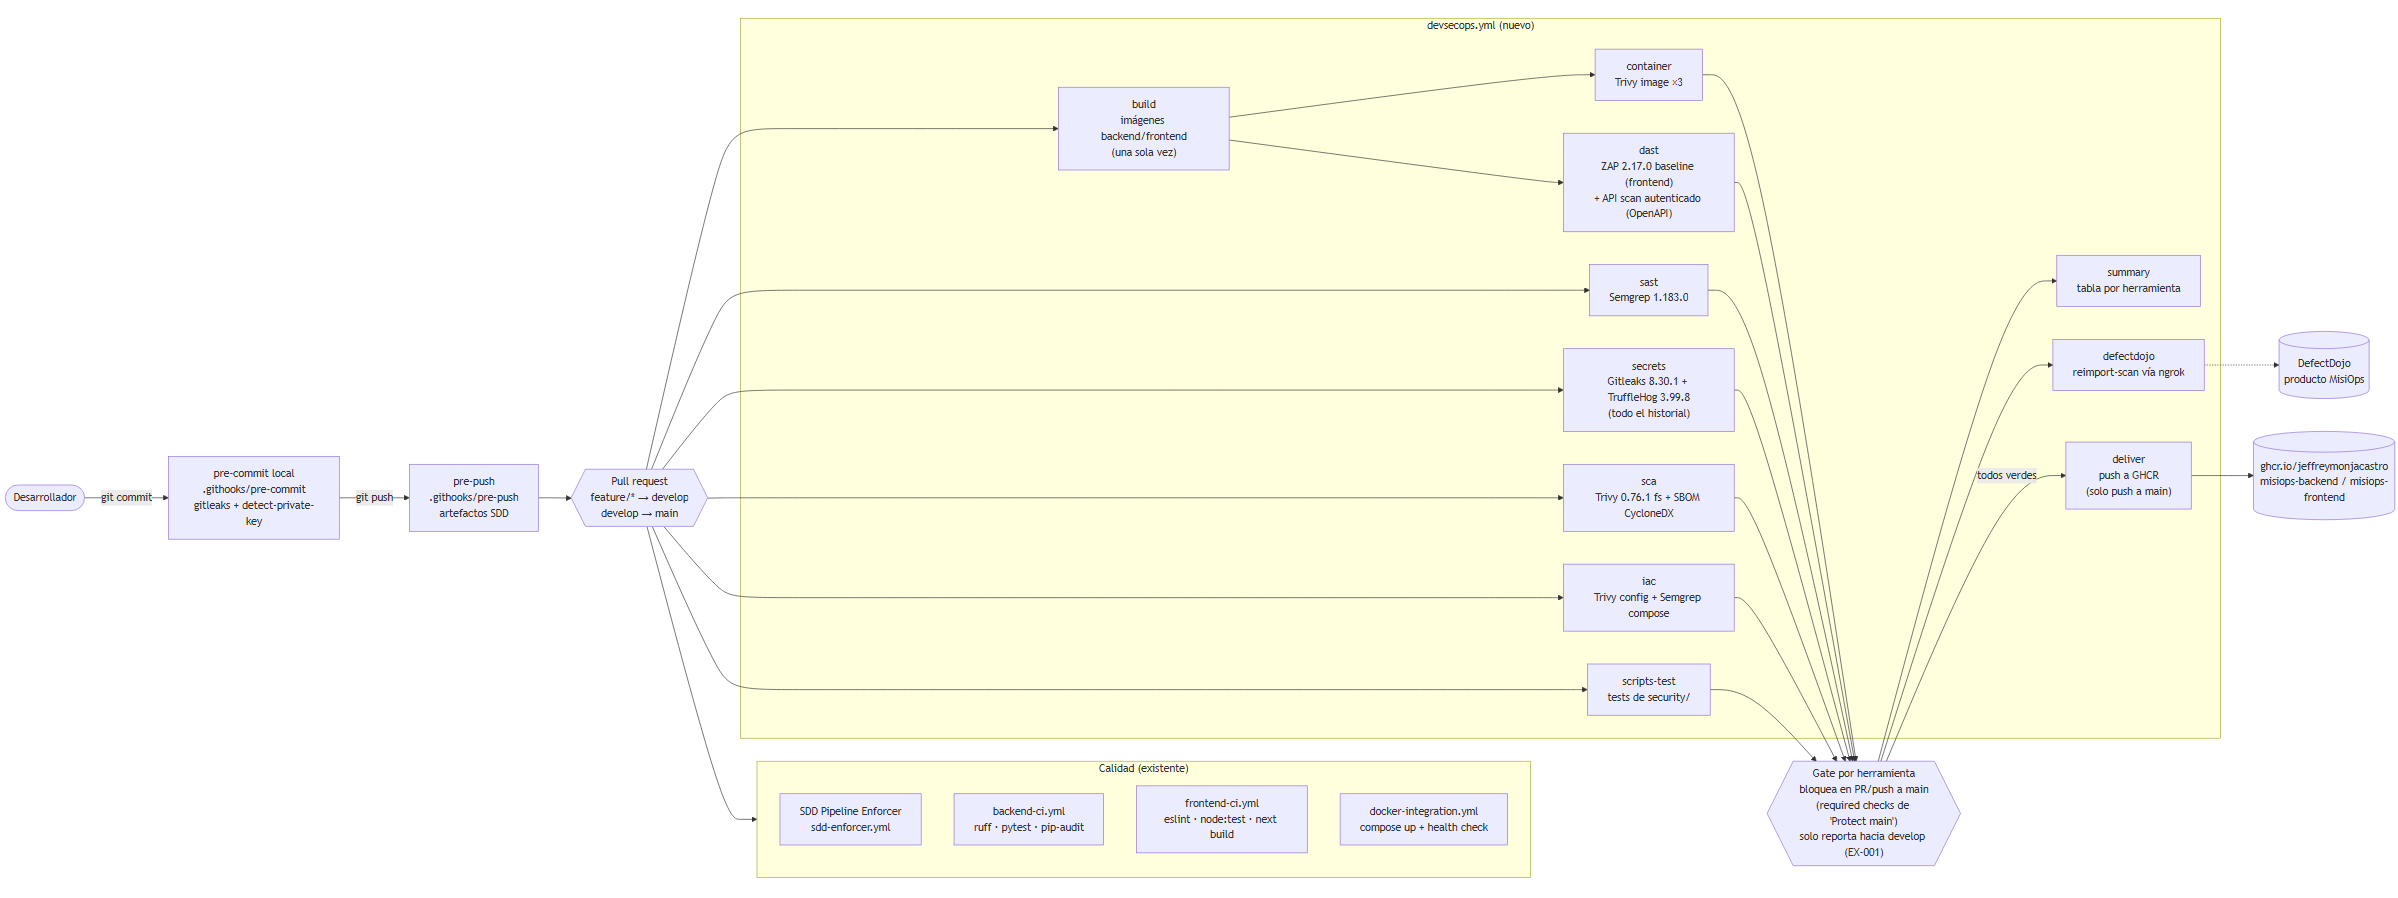
\includegraphics[width=\textwidth]{figures/devsecops/pipeline.png}
    \caption{Diagrama del pipeline CI/CD con las etapas de seguridad}
    \label{fig:pipeline}
\end{figure}

\begin{figure}[H]
    \centering
    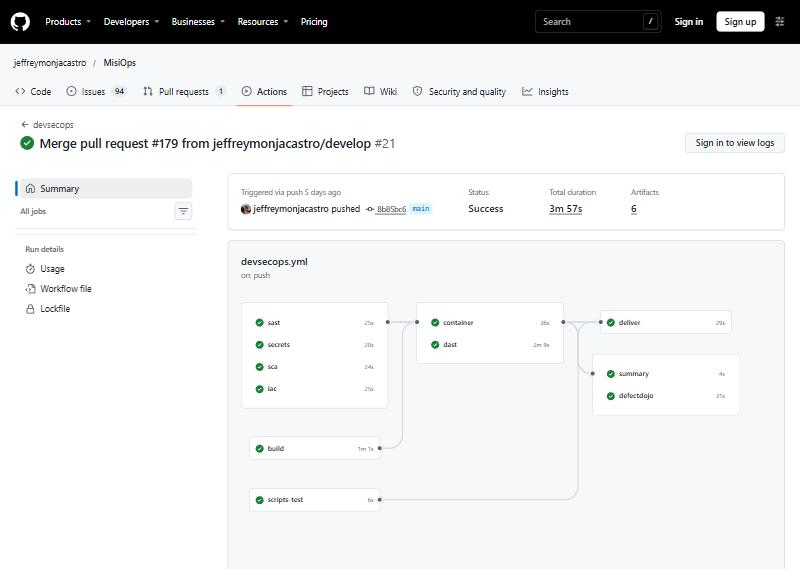
\includegraphics[width=\textwidth]{figures/devsecops/gh-actions-main.jpg}
    \caption{Corrida de \texttt{devsecops} sobre \texttt{main} tras el merge del PR \#179: todos los gates en verde, entrega a GHCR y subida a DefectDojo}
    \label{fig:gh-main}
\end{figure}

\subsubsection{Política de gates}

\begin{table}[H]
    \centering
    \small
    \caption{Condición de bloqueo de cada herramienta}
    \begin{tabularx}{\textwidth}{@{}p{4.5cm} X@{}}
        \toprule
        \textbf{Herramienta} & \textbf{Bloquea cuando...} \\
        \midrule
        Semgrep & Hay algún hallazgo de severidad \texttt{ERROR} \\
        Gitleaks / TruffleHog & Hay cualquier secreto que no esté en la lista de excepciones \\
        Trivy (dependencias e imágenes) & Hay CRITICAL o HIGH \textbf{con versión corregida disponible}; los que no tienen fix solo se reportan \\
        Trivy config / Semgrep compose & Hay alguna mala configuración HIGH o CRITICAL, o un hallazgo \texttt{ERROR} \\
        ZAP & Hay alguna alerta de riesgo High \\
        \bottomrule
    \end{tabularx}
\end{table}

El ruleset ``Protect main'' exige los checks \texttt{sast}, \texttt{secrets}, \texttt{sca}, \texttt{container}, \texttt{iac}, \texttt{dast} y \texttt{scripts-test}, además de una aprobación, y no tiene lista de \textit{bypass}. Para demostrar el bloqueo se abrió el PR de prueba \#131 hacia \texttt{main}: la rama era \texttt{develop} más un Dockerfile que corría como root a propósito (Trivy DS002, HIGH). El gate \texttt{iac} falló con \texttt{Trivy config: 1 blocking findings} y GitHub dejó el merge bloqueado. El PR se cerró sin merge.

\begin{figure}[H]
    \centering
    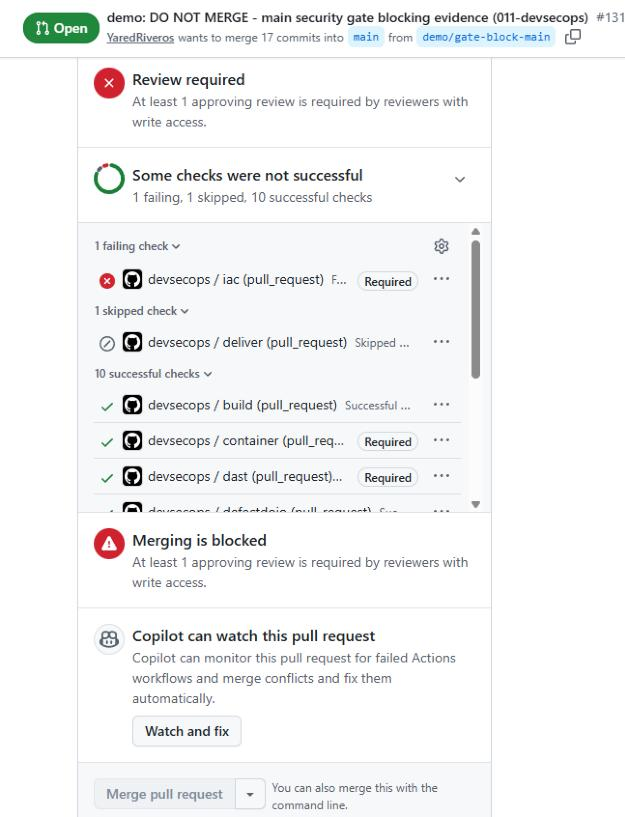
\includegraphics[width=0.85\textwidth]{figures/devsecops/main-merge-bloqueado.png}
    \caption{PR \#131 hacia \texttt{main}: el check requerido \texttt{iac} falla y el botón de merge queda deshabilitado}
    \label{fig:merge-bloqueado}
\end{figure}

\begin{figure}[H]
    \centering
    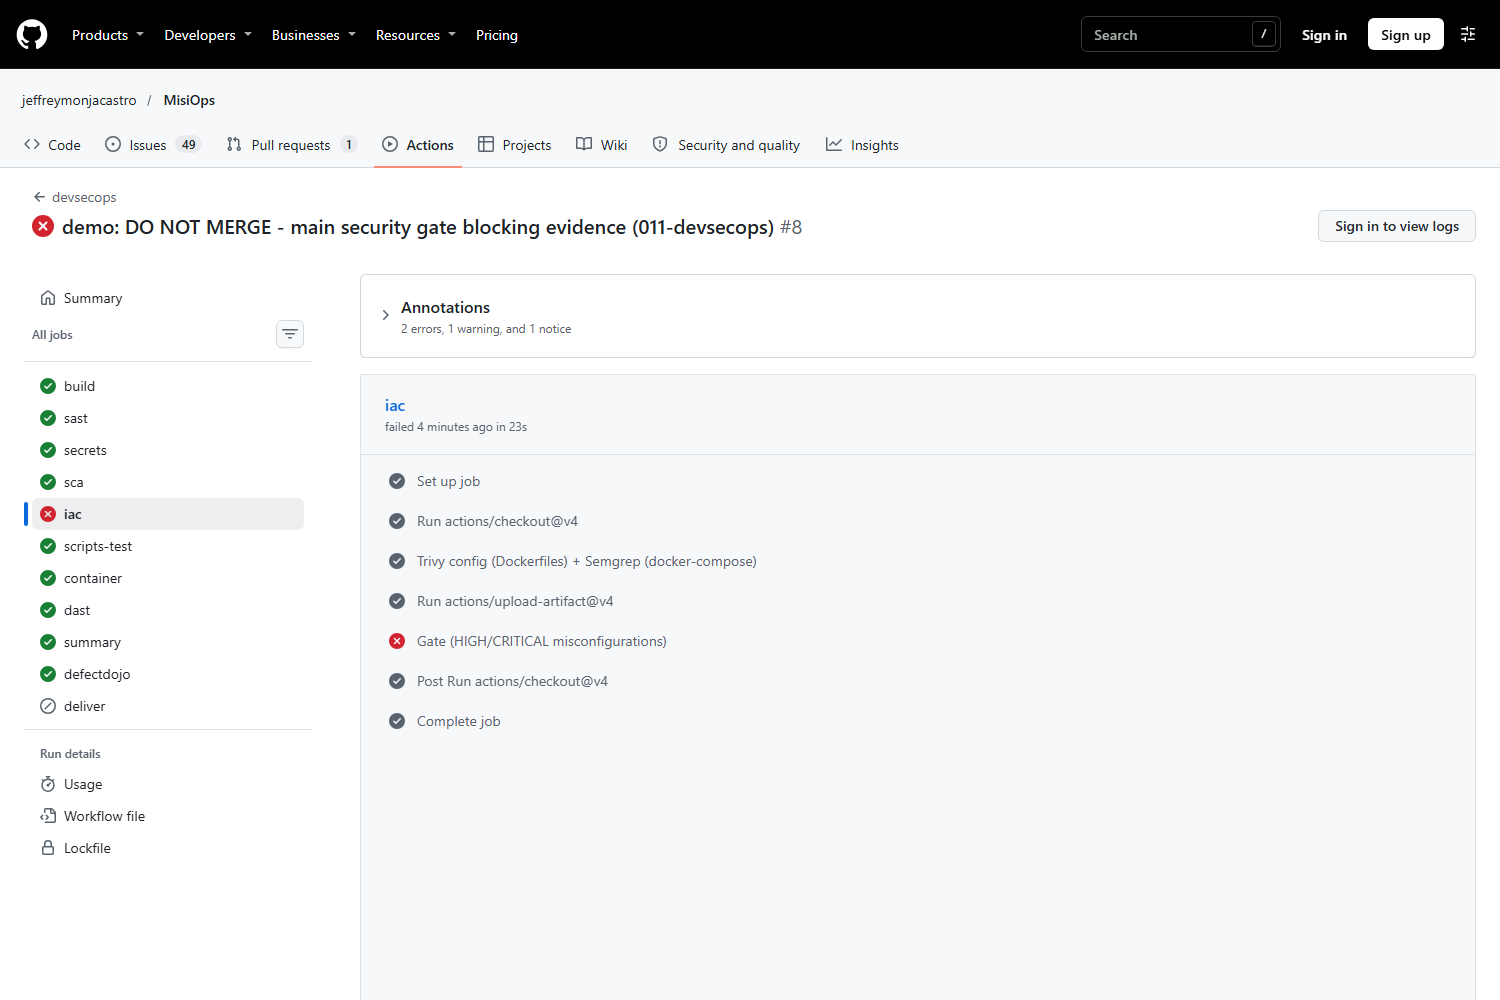
\includegraphics[width=\textwidth]{figures/devsecops/main-gate-iac-falla.png}
    \caption{Corrida del PR \#131: el gate \texttt{iac} detecta el hallazgo bloqueante}
    \label{fig:gate-iac}
\end{figure}

El gate funcionó igual en un caso real: el PR \#179, que promovía \texttt{develop} a \texttt{main}, quedó bloqueado cuando Debian publicó el fix de dos CVE HIGH de \texttt{zlib1g} en la imagen base del backend. Se corrigió con el PR \#180 (\texttt{apt-get upgrade} en el Dockerfile) y la promoción pasó.

Los scripts y archivos de configuración de la parte de seguridad se incluyen en el Anexo~\ref{anx:devsecops-config}.
